\renewcommand{\baselinestretch}{1.5}
\fontsize{12pt}{13pt}\selectfont

\chapter{绪论}\label{preface}

\section{研究背景}

当今阶段,无人机技术迅速发展,在单架无人机上配备的众多系统使单机已经能够执行各种各样的任务。如图\ref{fig-drone}所示,无人机上可以搭载机械臂来完成一些物体的抓取、运输任务;无人机上装配的设备不同,其实现的功能就不同;
单架无人机已经可以在自然灾害的搜救、对高空电力线路的检查、日常交通及场所的安全巡查、农业播种等场景发挥出巨大的作用。

\begin{figure}[!ht]
	\centering
	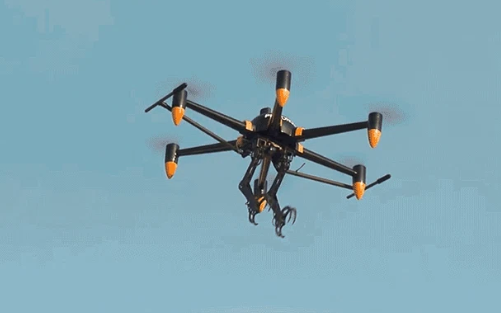
\includegraphics[width=0.6\textwidth]{drone.png}
	\caption{搭载机械臂系统的无人机} 
	\label{fig-drone}
\end{figure}

但是,单架无人机在执行任务时存在一定的局限性;
单架无人机拥有的计算设备最多仅有一个板载计算机,在面对多任务同时进行的情况时,难免会发生计算资源有限的情况;这种情景下无人机必须在计算的实时性和计算的质量之间做出抉择,无论采取任何一种策略都不利于任务的完成;
另一方面,单架无人机可搭载的设备数量和种类有限,这一定程度上是由于旋翼无人机气动效率不高,空气无法产生可观的向上的升力,其载重能力无法与利用空气升力飞行的固定翼飞机相比,因此对搭载设备的重量有严格限制,最终造成了无法配置较多设备和某些种类的设备;
且使用单机执行任务,即使无人机有着较低的故障率,但是一旦发生故障,很大程度上便意味着任务失败。
这些都意味着,在面对多种类的需求和复杂不可控的环境时,单架无人机可能无法发挥出其作用,无法确保任务的完成。
%但是,面对复杂的应用环境和多样化的需求,单架无人机受自身软硬件条件的限制,仍然具有一些局限性;
%为了弥补单架无人机的局限性,由多架相同或不同型号的无人机组成多无人机系统,即无人机集群,协同定位,共同完成任务;

为了弥补单架无人机的局限性,可以使用集群无人机的方案;即由若干架相同型号或根据任务需求搭配不同型号的无人机组成一个多无人机系统,进行协同定位,并借此完成任务。
%通过集群的方式,能最大地发挥无人机的优势,又能避免由于单架无人机执行任务不佳或失败造成的不良后果,提高任务执行效率,扩展新的任务执行方式,从而达到提高系统可靠性,增强任务执行效果的目的。

集群是使无人机的优势扩大的一种手段。首先可以有效降低任务的失误率和事故率;对于集群无人机任务而言,单架无人机出现故障对系统的影响比较小,因为系统可以具有任务重新规划能力,即系统中某些终端退出任务后,系统仍有能力重新组织分配当前可用资源,因此单架无人机的故障甚至是事故对任务的负面影响被降低了。
其次是在实际应用中的任务执行效率;对于固定范围场景的探索任务,单架无人机可能需要运动数个来回才能得到对场景的识别任务,但集群使用多终端,一方面可以扩展探索范围,另一方面可以提升任务效率。
集群的方式还可以大幅度拓展其任务执行方式;单机由于携带设备的局限性,对于多设备需求的任务,往往需要多个起降循环,而集群系统则可以配置不同传感器和设备的无人机,一次性地完成任务,这很大程度上扩展了任务执行的途径。
因此,集群无人机可以降低任务失败率,提升多无人机系统鲁棒性,有效提升任务完成率。

无论何种任务,无人机建立对未知环境的感知、获得自身的位置和姿态并获得自主导航能力,是任务成功的前提和关键。
尽管GPS对于掌握无人机的位置有巨大的帮助,但仍存在普适性有限和准确度不高的问题;在一些特定场景下,比如室内狭小空间,对定位精度要求很高,GPS定位的局限性就被显露出来。或是GPS信号弱的情况下,无人机如果仅依靠GPS获得定位信息,则可能完全无法进行工作。

为了弥补这一缺陷,可以使用SLAM技术;
SLAM技术,即同时完成定位与建图的任务,已有较为系统的理论和研究;SLAM于20世纪90年代左右由 Smith、Cheeseman 和Self提出。
SLAM是指将机器人放置在陌生环境中,令其从未知位置开始运动,在行进中根据解算出的当前位置和初步构建的地图获取自身位置信息,基于此建立增量式地图,从而达成使机器人获得自主定位和导航能力的目标\cite{王晨捷2020无人机视觉}。
因此,SLAM可以仅通过自身携带的传感器,来完成这一任务,同时达到一定的精度;


%SLAM指的是机器人在未知环境中从一个未知位置开始移动,在移动过程中根据位置和地图进行自身定位,同时在自身定位的基础上建造增量式地图,实现机器人的自主定位和导航。由于其重要的理论与应用价值,被很多学者认为是实现真正全自主移动机器人的关键。


SLAM主要分为视觉SLAM、激光SLAM、融合SLAM和新颖SLAM。


对于视觉SLAM,即用相机完成同时定位与建图的任务。由于相机造价相对较低、电量消耗相对较少、能够获取环境的大量信息,因此相机成为了完成定位与建图任务常用的传感器。视觉SLAM主要有五个步骤,传感器信息读取、视觉里程计(Visual Odometry)、后端优化(Optimization)、回环检测(Loop Closing)、建图(Mapping。对于静态、刚体、光照变化不明显、且没有过多人为干扰的场景,视觉SLAM技术已经十分成熟。当前比较好的方案有ORB-SLAM;其在对特征点的描述上做了很大创新,相比于SIFT(尺度不变特征变换,Scale-invariant feature transform)的大计算量和对GPU的特殊需求、FAST关键点描述没有描述子的缺点,ORB改进了FAST的检测子,为其增加了方向性,并且采用了二进制描述子BRIEF(Binary Robust Independent Elementary Feature) \cite{rublee2011orb}。


对于激光SLAM,主要有两种传感器,单线束激光雷达和多线束激光雷达;单线束激光雷达即2D雷达,2D激光雷达的扫描范围比较单一,角度有限,因此比较适合仅平面运动的机器人的定位与建图,对应的经典算法如GMapping;多线束雷达即3D雷达,其获取的信息包含距离和角度,能够还原出目标的三维点云,且不受光照影响,缺点是造价比较昂贵且易受不良天气影响\cite{杨明2000基于激光雷达的移动机器人环境建模与避障},对应的经典算法如谷歌提出的Cartographer。


对于融合SLAM,常见的有视觉和惯性的融合,即相机+IMU(inertial measurement unit,惯性测量单元,包含加速度计和角加速度计)等的多传感器融合;IMU的工作原理是对加速度的积分、初始速度和起始位置进行混合运算,得到运动轨迹和位姿。但是其容易产生漂移(Drift),并且这种累积误差会随时间增加\cite{avrutov2017calibration}。


对于VIO(视觉惯性里程计),即上文提到的由相机和惯性测量单元组成的融合传感器,根据融合的框架可以分为松耦合和紧耦合两种。松耦合中对相机关键帧数据的视觉运动估计和对IMU测量数据的运动估计是两个独立的模块,计算时互不干涉;计算完成后将其轨迹结果按一定的方法进行融合。紧耦合则是共同使用相机视觉数据和惯导运动估计数据,共同完成对一组变量的估计\cite{qin2018vins};因此其算法更加复杂,且传感器之间的噪声也会相互影响,但是具有更好的效果,也是目前阶段研究的重点方向。这方向上好的方案有VINS-fusion。


对于新颖SLAM,比如语义SLAM;使用神经网络的语义分割、目标检测方法,从图像到位姿,使用其语义分割的结果来完成点云地图的建立和场景识别。语义SLAM能够探测出图像中的各个物体,并且能得到在图像中的位置,可以节省传统的人工标定物品的成本,方便机器人的自主理解能力和简便的人机交互\cite{任伟建2022移动机器人同步定位与建图技术综述}。

尽管单终端SLAM已经发展地比较成熟,但是单平台SLAM受到传感器性能的限制,存在两点不足:一是测量距离受限,单平台常用的传感器如激光雷达,其最远有效距离为200米,不能够满足大场景定位建图的需要,任务效率比较低;二是单平台构建出的三维点云相对稀疏,不能表现出足够的场景信息\cite{高家隆2019多无人机协同定位与建图技术研究}。

因此集群无人机协同SLAM方案有望解决单机存在的制约问题,主要表现在两个方面:一是多机意味着多传感器,能在大范围场景进行同时定位与建图;二是多机协同SLAM可以通过建图覆盖的检测,构建更加稠密和精细的点云地图。

目前单机同时定位与建图已经相对成熟,但是多机SLAM由于其控制复杂、数据传输量大、信息处理速度受限、关键数据融合效率低等问题,仍然大量的研究和实验。

\section{国内外研究现状}

%国内外研究现状
集群无人机或多设备上的协同SLAM方案研究上,目前国内比较成熟的有浙江大学FAST-LAB实验室的通过装配有D345双目相机的无人机进行在密集障碍物环境下的分布式无人机编队行进,如图\ref{fig-fastlab}所示;其弱化了SLAM的内容,但实际其使用的IMU+深度相机信息的视觉里程计和建图仍属于SLAM的工作内容,SLAM在其中承担了较为底层的工作。

\begin{figure}[!ht]
	\centering
	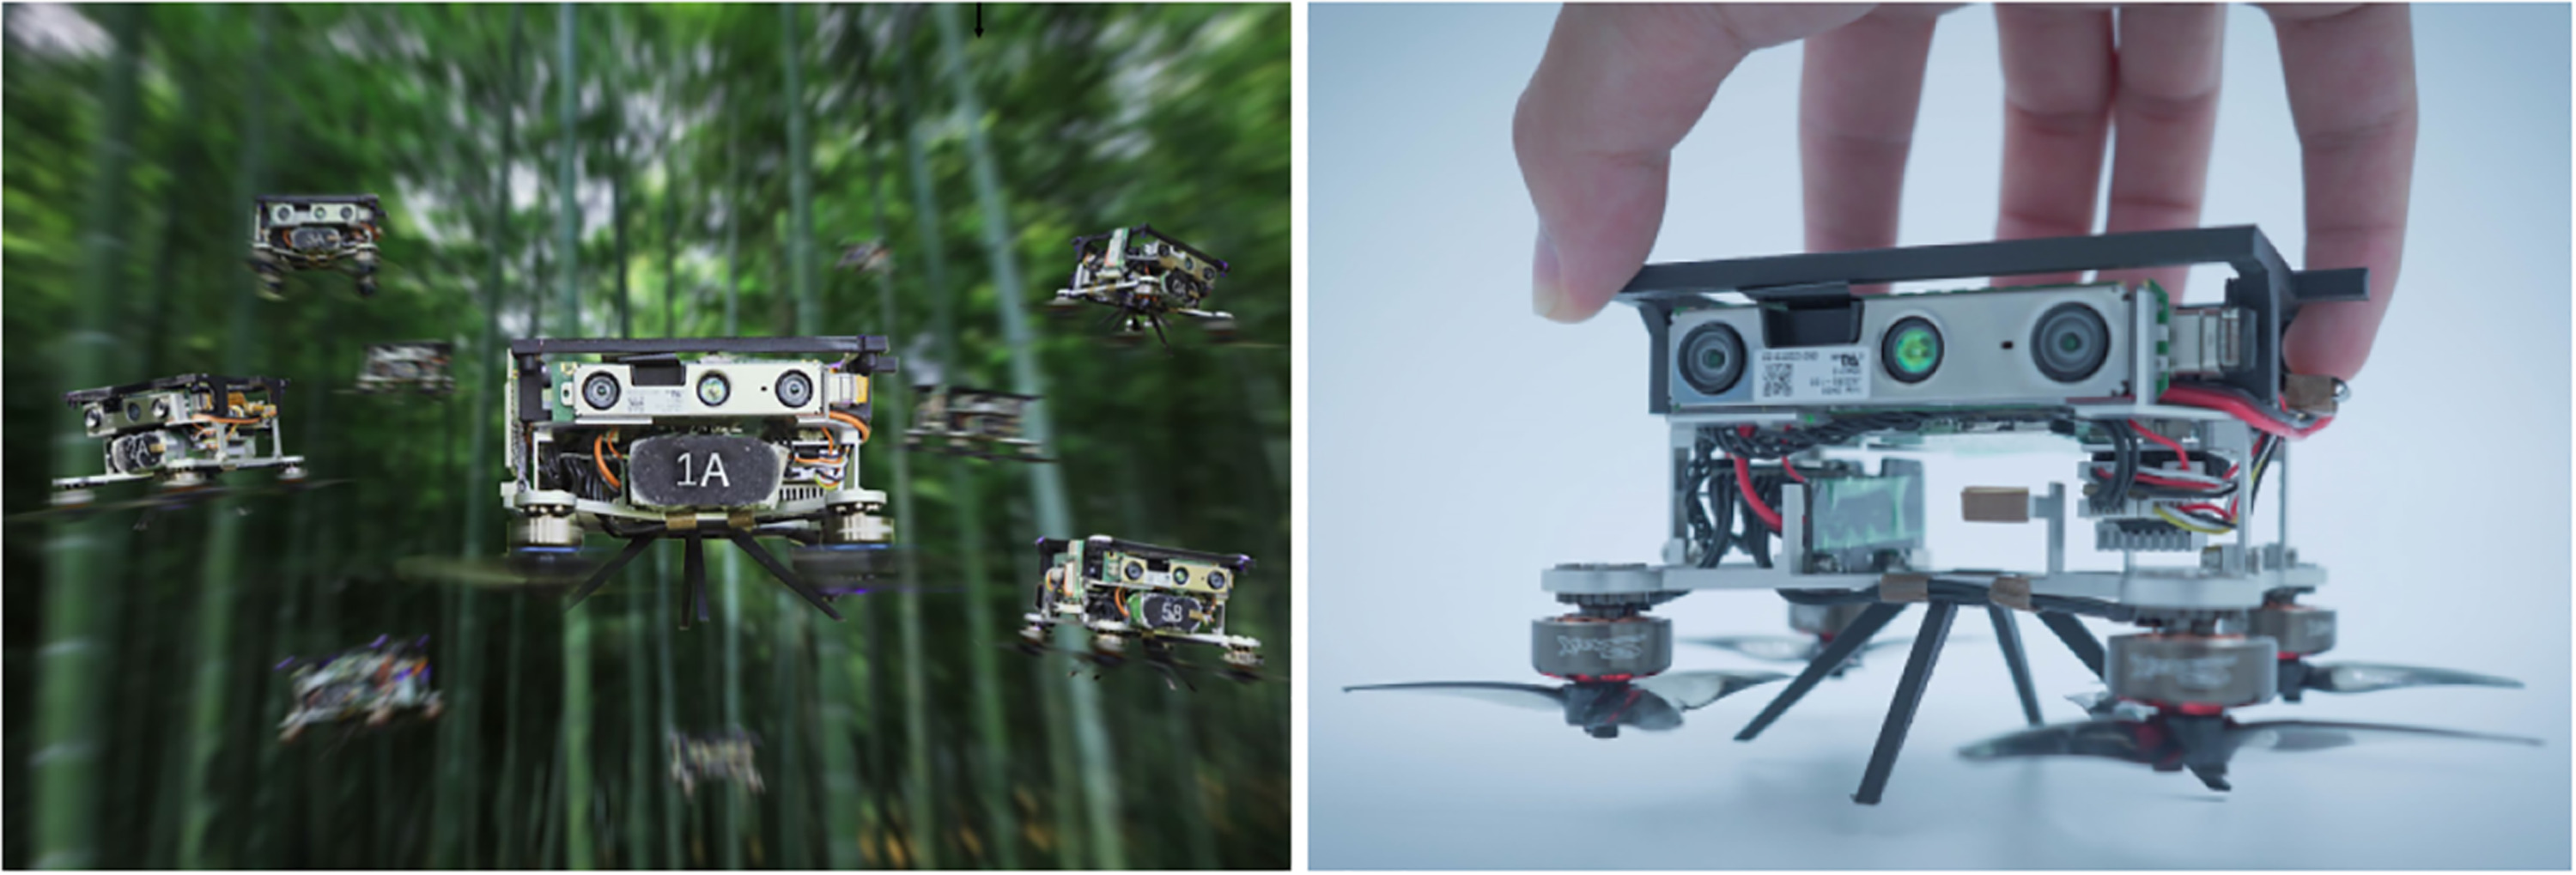
\includegraphics[width=0.9\textwidth]{fastlab.jpg}
	\caption{FAST-LAB智能无人机集群} 
	\label{fig-fastlab}
\end{figure}

除此之外,香港科技大学的空中机器人组正在开展Omni-swarm的研究,其内容可以总括为一套使用视觉惯性里程计和UWB单元的集群状态估计系统。具体来说,该团队使用全方向的视觉+惯性里程计和UWB模块的,完成对分布式多机的状态估计;在SLAM前端的设计上,使用了全方向的感知前端;在多无人机的SLAM任务中,将多机得到的地图在本地进行优化处理,得到一致的地图;如图\ref{fig-omni}所示,各机的状态估计使用前端VIO的测量值与后端图优化的值结合,而UWB模块的引入更加增加了定位的精确度,使得该系统最终得以达到厘米级的状态估计精度,并且还能够保证世界坐标系中无人机运动轨迹的连续性;该团队用实验证明了使用其方法可以为室内无人机避障和防撞提供足够的支持,由此可以构建真正意义上全自主的无人机集群\cite{omniSwarm}。此外,西北工业大学的PI-LAB实验室也正在开展集群无人机相关领域的研究。

\begin{figure}[!ht]
	\centering
	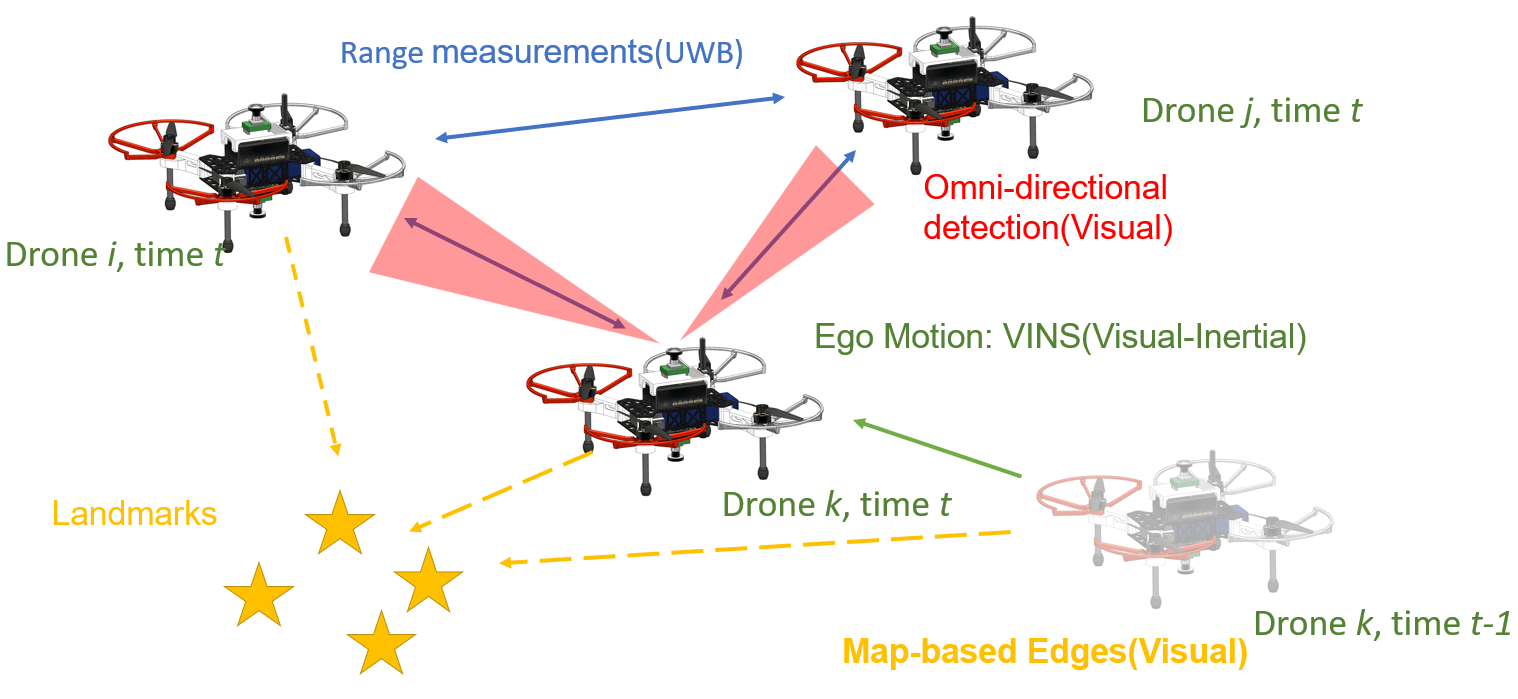
\includegraphics[width=0.9\textwidth]{omni.png}
	\caption{Omni Swarm的融合测量方法} 
	\label{fig-omni}
\end{figure}

国外则拥有较多的研究,新加坡国立大学在2012年就提出了CoSLAM,根据视图的重叠构建全局地图\cite{zou2012coslam}。
苏黎世联邦理工大学提出的ccm-slam系统,就是一个以客户端和服务器模型构建的中心式多机协同SLAM方案,其使用的底层SLAM方案仍然是ORB-SLAM2\cite{schmuck2019ccm};在这之后,又提出了CO-VINS方案,也是一种协同式的SLAM方案,但使用的底层代码是ORB-SLAM3\cite{9585827},相比于ccm的特点是加入了惯性测量元件的信息。

\section{研究内容及论文结构}
本文研究目标旨在实现一套能够在室内高精度环境或GPS拒止环境下使用视觉进行多机定位和大范围建图的多无人机协同SLAM的方案;其中:

\begin{enumerate}
	\item 在SLAM方面:掌握一些优秀的开源方案,选择各自优点做出一定的融合。并且有一套针对地图融合的方法。
	\item 在仿真方面:在ROS的gazebo仿真平台中实现一定的集群控制方法,能够控制多个无人机协同完成同时定位与建图的任务。
	\item 在真机方面:实现单机的视觉SLAM;在安全的前提下实现双机协同SLAM,将仿真环境下的协同SLAM算法在真机上完成验证,得到场景地图
\end{enumerate}

本研究内容是多机协作进行定位与建图,多机协同SLAM能大大提高任务进行的效率,但由于无人机数量多,协同上存在一定困难;研究内容分为三个模块:SLAM模块、仿真模块和真机模块。

SLAM模块的主要内容是实现一套可协作的SLAM方案,实现的步骤有:

\begin{enumerate}
	\item 研究传统的视觉SLAM的特征点提取、匹配、初始化、后端优化等技术,研究机器人的位姿估计技术;研究并了解SLAM技术的整体框架
	\item 研究CCM-SLAM方案,重点研究其协同的机制和方法,服务端到子端的信息传递和接口设计等
	\item 研究VINS-Fusion方案中的VIO方法,研究如何利用IMU与相机数据联合进行更加准确的位姿估计
\end{enumerate}

仿真模块的主要内容是在ROS的gazebo中研究如何实现多机协同的同时定位与建图,实现的步骤有:

\begin{enumerate}
	\item 首先研究PX4和MAVROS之间的通信方式,ROS的话题发布和订阅方式,研究如何用程序解锁一架无人机、使其进入Offboard模式、起飞悬停并降落
	\item 研究如何用程序发布话题,控制无人机按照航路点飞行
	\item 研究如何构建多机的仿真环境,如何对多机进行控制,其控制策略的选择,即集中式或分布式的多机编队控制
	\item 研究如何更改无人机的定位设置,将其从GPS定位改为视觉SLAM定位;并且完成单机的摄像头内容读取
	\item 研究如何在gazebo中载入其他场景,在场景中控制无人机飞行,并且对拍摄到的画面进行建图,完成自身定位
	\item 研究如何在gazebo中完成多机基于视觉的同时定位与建图,并且拼合地图,用第三方软件显示;研究多机的联合优化与协同方法
\end{enumerate}

真机模块的主要内容是控制无人机的协同飞行及通信,实现的步骤有:

\begin{enumerate}
	\item 研究无人机通过MAVROS,MAVLINK与地面站的通信方法,尤其是用于SLAM的关键数据的传输
	\item 研究多无人机与地面站之间的、多无人机之间的数据传输
	\item 研究多无人机之间的可变基线控制技术,如何设计一个详细的算法控制基线距离
\end{enumerate}

基于研究内容的层级关系,本论文的结构主要由四层构成,如图\ref{fig1}所示。
\vspace{10pt}
\begin{figure}[!ht]
\centering
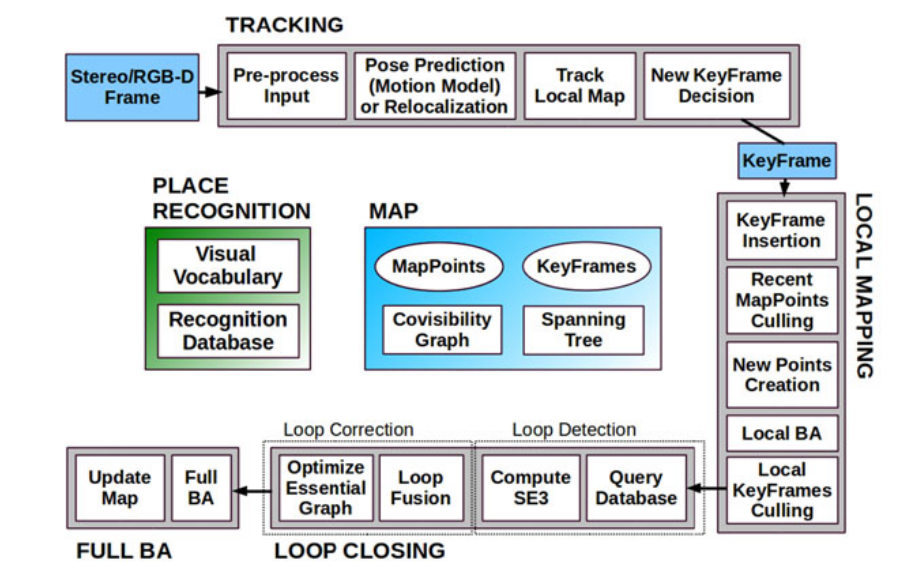
\includegraphics[width=0.8\textwidth]{structure.png}
\caption{论文结构 }
\label{fig1}
\end{figure}


第\ref{preface}章:主要介绍本文相关研究背景和现状;根据现阶段存在的问题,引出本文的研究方向和内容;从宏观的角度概括本文的内容,并且对问题做出概述。

第\ref{introduction}章:主要介绍研究中用到的ROS(Robotics Operating System,机器人操作系统)和PX4 AutoPilot飞控软件系统。

第\ref{System Overview}章:主要介绍SLAM的原理和作用,SLAM系统的基本流程,优秀的开源SLAM方案和地图融合的设计。

第\ref{Simulation}章:主要介绍仿真实验的情况,在ROS的gazebo环境中进行。

第\ref{experiment}章:主要介绍真机实验的情况,并且做出相应的评估。

第\ref{conclusion}章:总结本文研究中的创新点和有待改进之处,提出进一步研究的大致方向,展望未来的研究工作。

